%%%%%%%%%%%%%%%%%%%%%%%%%%%%%%%%%%%%%%%%%%%%%%%%%%%%%%%%%%%%%%%
%
% Welcome to Overleaf --- just edit your LaTeX on the left,
% and we'll compile it for you on the right. If you give
% someone the link to this page, they can edit at the same
% time. See the help menu above for more info. Enjoy!
%
% Note: you can export the pdf to see the result at full
% resolution.
%
%%%%%%%%%%%%%%%%%%%%%%%%%%%%%%%%%%%%%%%%%%%%%%%%%%%%%%%%%%%%%%%
% Decision tree
% Author: Stefan Kottwitz
% https://www.packtpub.com/hardware-and-creative/latex-cookbook

\documentclass[border=10pt]{standalone} 

\usepackage[utf8]{inputenc}

\usepackage{tikz}
\tikzset{
  treenode/.style = {shape=rectangle, rounded corners,
                     draw, align=center,
                     top color=white, bottom color=blue!20},
  root/.style     = {treenode, font=\normalsize, bottom color=red!30},
  env/.style      = {treenode, font=\ttfamily\small},
  edge/.style      = {font=\ttfamily\small},
  dummy/.style    = {circle,draw}
}
\begin{document}
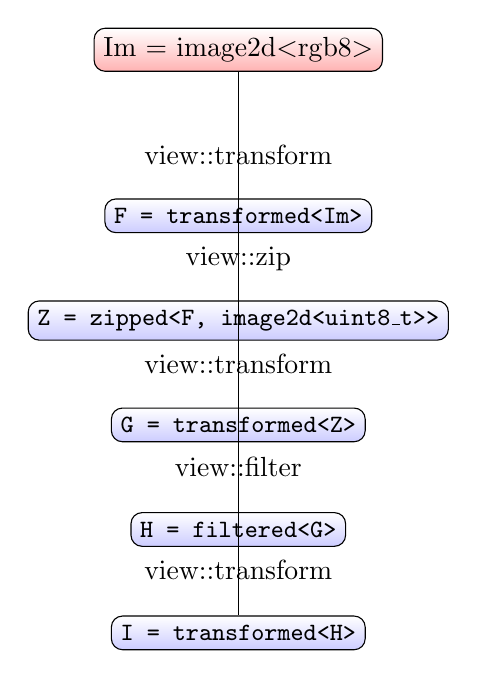
\begin{tikzpicture}
  [
    sibling distance        = 3em,
    level distance          = 6em,
    edge from parent/.style = {draw},
  ]
  \node [root] {Im = image2d\textless rgb8\textgreater}
  child { node [env] {F = transformed<Im>}
      edge from parent node [below] {view::transform}
      child { node [env] {Z = zipped<F, image2d<uint8\_t>>}
          edge from parent node [below] {view::zip}
          child { node [env] {G = transformed<Z>}
              edge from parent node [below] {view::transform}
              child { node [env] {H = filtered<G>}
                  edge from parent node [below] {view::filter}
                  child { node [env] {I = transformed<H>}
                      edge from parent node [below] {view::transform}
                    } } } } };
\end{tikzpicture}
\end{document}